%% abtex2-modelo-trabalho-academico.tex, v-1.9.2 laurocesar
%% Copyright 2012-2014 by abnTeX2 group at http://abntex2.googlecode.com/ 
%%
%% This work may be distributed and/or modified under the
%% conditions of the LaTeX Project Public License, either version 1.3
%% of this license or (at your option) any later version.
%% The latest version of this license is in
%%   http://www.latex-project.org/lppl.txt
%% and version 1.3 or later is part of all distributions of LaTeX
%% version 2005/12/01 or later.
%%
%% This work has the LPPL maintenance status `maintained'.
%% 
%% The Current Maintainer of this work is the abnTeX2 team, led
%% by Lauro César Araujo. Further information are available on 
%% http://abntex2.googleco@misc{MarileneCarneiroMatos,

%%
%% This work consists of the files abntex2-modelo-trabalho-academico.tex,
%% abntex2-modelo-include-comandos and abntex2-modelo-references.bib
%%
% ------------------------------------------------------------------------
% ------------------------------------------------------------------------
% abnTeX2: Modelo de Trabalho Academico (tese de doutorado, dissertacao de
% mestrado e trabalhos monograficos em geral) em conformidade com 
% ABNT NBR 14724:2011: Informacao e documentacao - Trabalhos academicos -
% Apresentacao
% ------------------------------------------------------------------------
% ------------------------------------------------------------------------


%Testando o git

\documentclass[
	% -- opções da classe memoir --
	12pt,				% tamanho da fonte
	openright,			% capítulos começam em pág ímpar (insere página vazia caso preciso)
	oneside,			% para impressão em verso e anverso. Oposto a oneside
	a4paper,			% tamanho do papel. 
	% -- opções da classe abntex2 --
	%chapter=TITLE,		% títulos de capítulos convertidos em letras maiúsculas
	%section=TITLE,		% títulos de seções convertidos em letras maiúsculas
	%subsection=TITLE,	% títulos de subseções convertidos em letras maiúsculas
	%subsubsection=TITLE,% títulos de subsubseções convertidos em letras maiúsculas
	% -- opções do pacote babel --
	english,			% idioma adicional para hifenização
	brazil				% o último idioma é o principal do documento
	]{abntex2}

% ---
% Pacotes básicos 
% ---
\usepackage{unitins}
% \usepackage{lmodern}			% Usa a fonte Latin Modern			
% \usepackage[T1]{fontenc}		% Selecao de codigos de fonte.
 \usepackage[utf8]{inputenc}		% Codificacao do documento (conversão automática dos acentos)
 \usepackage{lastpage}			% Usado pela Ficha catalográfica
 \usepackage{indentfirst}		% Indenta o primeiro parágrafo de cada seção.
 \usepackage{color}				% Controle das cores

\usepackage{graphicx}			% Inclusão de gráficos
\usepackage{subfig}
\usepackage{microtype} 			% para melhorias de justificação
\usepackage{soul}
\usepackage{amssymb}
\usepackage{amsmath}
\usepackage{spreadtab}
\usepackage{multirow}
\usepackage{amsthm}
\usepackage{url}
% \usepackage[portuguese, ruled, linesnumbered]{algorithm2e}


% ---
		
% ---
% Pacotes adicionais, usados apenas no âmbito do Modelo Canônico do abnteX2
% ---
		% para geração de dummy text
% ---

% ---
% Pacotes de citações
% ---

%\usepackage[brazilian,hyperpageref]{backref}	 % Paginas com as citações na bibl
\usepackage[alf,abnt-etal-list=2 ]{abntex2cite}	% Citações padrão ABNT


\usepackage[table]{xcolor}
\definecolor{lightgray}{gray}{0.9}
\graphicspath{{imagens/}}

\theoremstyle{theorem}
\newtheorem{teo}{Teorema}[chapter]
\newtheorem{lema}[teo]{Lema}
\theoremstyle{definition}
\newtheorem{defi}[teo]{Definição}

% --- 
% CONFIGURAÇÕES DE PACOTES
% --- 

% ---
% Configurações do pacote backref
% Usado sem a opção hyperpageref de backref
%\renewcommand{\backrefpagesname}{Citado na(s) página(s):~}
% Texto padrão antes do número das páginas
%\renewcommand{\backref}{}
% Define os textos da citação
%\renewcommand*{\backrefalt}[4]{
%	\ifcase #1 %
%		Nenhuma citação no texto.%
%	\or
%		Citado na página #2.%
%	\else
%		Citado #1 vezes nas páginas #2.%
%	\fi}%
% ---

% ---
% Informações de dados para CAPA e FOLHA DE ROSTO
% ---
\titulo{PROPOSTA DE UM MODELO DE IMPLANTAÇÃO PARA APLICAÇÃO EXTERNA UTILIZANDO CONCEITOS DEVOPS}
\autor{MATHEUS JOSÉ ALVES SILVA SANTOS}
\local{Palmas}
\data{2018}
\orientador{Prof. Me. Douglas Chagas da Silva}
\instituicao{%
  Universidade Estadual do Tocantins
  \par
  Curso de Sistemas de Informação
  }
\tipotrabalho{Trabalho de Conclusão de Curso (Graduação)}
% O preambulo deve conter o tipo do trabalho, o objetivo, 
% o nome da instituição e a área de concentração 
\preambulo{Projeto apresentado como requisito para aprovação na disciplina de Estágio Supervisionado do Curso de Sistemas de Informações da Universidade Estadual do Tocantins- UNITINS, sob a orientação do professor Me. Douglas Chagas.}

% ---


% ---
% Configurações de aparência do PDF final

% alterando o aspecto da cor azul
\definecolor{blue}{RGB}{41,5,195}

% informações do PDF
\makeatletter
\hypersetup{
     	%pagebackref=true,
		pdftitle={\@title}, 
		pdfauthor={\@author},
    	pdfsubject={\imprimirpreambulo},
	    pdfcreator={LaTeX with abnTeX2},
		pdfkeywords={Algoritmo}{trabalho acadêmico}, 
		colorlinks=true,       		% false: boxed links; true: colored links
    	linkcolor=blue,          	% color of internal links
    	citecolor=blue,        		% color of links to bibliography
    	filecolor=magenta,      		% color of file links
		urlcolor=blue,
		bookmarksdepth=4
}
\makeatother
% --- 

% --- 
% Espaçamentos entre linhas e parágrafos 
% --- 

% O tamanho do parágrafo é dado por:
\setlength{\parindent}{1.3cm}

% Controle do espaçamento entre um parágrafo e outro:
\setlength{\parskip}{0.2cm}  % tente também \onelineskip

% ---
% compila o indice
% ---
\makeindex
% ---

% ----
% Início do documento
% ----
\begin{document}

% Retira espaço extra obsoleto entre as frases.
\frenchspacing 

% ----------------------------------------------------------
% ELEMENTOS PRÉ-TEXTUAIS
% ----------------------------------------------------------
% \pretextual
% ----------------------------------------------------------

% ----------------------------------------------------------
% ELEMENTOS PRÉ-TEXTUAIS
% ----------------------------------------------------------
% \pretextual

% ---
% Capa
% ---
\imprimircapa
% ---

% ---
% Folha de rosto
% (o * indica que haverá a ficha bibliográfica)
% ---
\imprimirfolhaderosto
% ---

% ---
% Inserir folha de aprovação
% ---

% Isto é um exemplo de Folha de aprovação, elemento obrigatório da NBR
% 14724/2011 (seção 4.2.1.3). Você pode utilizar este modelo até a aprovação
% do trabalho. Após isso, substitua todo o conteúdo deste arquivo por uma
% imagem da página assinada pela banca com o comando abaixo:
%
% \includepdf{folhadeaprovacao_final.pdf}
%
\begin{folhadeaprovacao}

  	
  	
  	\begin{center}
  		
\includegraphics[width=1\textwidth]{imagens/unitins.png}
  		\ABNTEXchapterfont\Large   CURSO DE SISTEMAS DE INFORMA{\c{C}}{\~{A}}O
  		
  		\par
  		\vspace*{1cm}     
  		{\ABNTEXchapterfont\bfseries\large \expandafter\MakeUppercase{\imprimirtitulo}  \vspace*{1cm}    }
  		\par
  		{\large \expandafter\MakeUppercase{\imprimirautor}}
  		%\vspace*{\fill}
  		\par
  		\vspace*{1cm}     
  		\hspace{.45\textwidth}
  		\begin{minipage}{.5\textwidth}
  			\small\imprimirpreambulo
  			
  		\end{minipage}%
  	%	\vspace*{\fill}
  	\end{center}
  
        
  
   \assinatura{\textbf{\imprimirorientador} \\ Orientador} 
   \assinatura{\textbf{Professor} \\ Convidado 1}
   \assinatura{\textbf{Professor} \\ Convidado 2}
   %\assinatura{\textbf{Professor} \\ Convidado 3}
   %\assinatura{\textbf{Professor} \\ Convidado 4}
      
   \begin{center}
    \vspace*{0.5cm}
    {\large\imprimirlocal}
    \par
    {\large\imprimirdata}
    \vspace*{1cm}
  \end{center}
  
\end{folhadeaprovacao}
% ---

% ---
% Dedicatória
% ---
\begin{dedicatoria}
   \vspace*{\fill}
   \centering
   \noindent
   \textit{ Este trabalho é dedicado à minha família, pelo apoio incondicional.} \vspace*{\fill}
\end{dedicatoria}
% ---

% ---
% Agradecimentos
% --- Es
\begin{agradecimentos}
Aos meus pais que sempre me incentivaram a superar as dificuldades. 
Aos meus amigos de jornada, por não me deixarem desistir.


\end{agradecimentos}
% ---

% ---
% Epígrafe
% ---
\begin{epigrafe}
    \vspace*{\fill}
	\begin{flushright}
		\textit{``Não vos amoldeis às estruturas deste mundo, \\
		mas transformai-vos pela renovação da mente, \\
		a fim de distinguir qual é a vontade de Deus: \\
		o que é bom, o que Lhe é agradável, o que é perfeito.\\
		(Bíblia Sagrada, Romanos 12, 2)}
	\end{flushright}
\end{epigrafe}
% ---

% ---
% RESUMOS
% ---

% resumo em português
\setlength{\absparsep}{18pt} % ajusta o espaçamento dos parágrafos do resumo
\begin{resumo}
resumo
 

 \textbf{Palavras-chaves}: .
 
\end{resumo}

% resumo em inglês
\begin{resumo}[Abstract]
 \begin{otherlanguage*}{english}
 abstract
   \vspace{\onelineskip}
 
   \noindent 
   \textbf{Key-words}:.
 \end{otherlanguage*}
\end{resumo}


% ---
% inserir lista de ilustrações
% ---
\pdfbookmark[0]{\listfigurename}{lof}
\listoffigures*
% ---

% ---
% inserir lista de tabelas
% ---
\newpage
\pdfbookmark[0]{\listtablename}{lot}
\newpage
\listoftables*
\cleardoublepage
% ---

% ---
% inserir lista de abreviaturas e siglas
% ---
\begin{siglas}
  \item POM - Problema de Otimização Multiobjetivo.
  
  
  
\end{siglas}
% ---


% ---
% inserir o sumario
% ---
\pdfbookmark[0]{\contentsname}{toc}
\tableofcontents*
\cleardoublepage
% ---



% ELEMENTOS TEXTUAIS
% ---------------------------------[!htb]-------------------------
%\textual

%Capitulos
% ----------------------------------------------------------
% Introdução (exemplo de capítulo sem numeração, mas presente no Sumário)
% ----------------------------------------------------------

\chapter{Introdução}\label{intro}

Aqui vai a introdução



\section{Objetivos}
\subsection{Objetivo Geral }
Apresentar um modelo de arquitetura de aplicação externa para entrega contínua baseada na visão DevOps.



\begin{comment}
Este é um comentário
\end{comment}

\subsection{Objetivos Específicos}
\begin{itemize}
\item Diferenciar o modelo tradicional de deploys e a visão DevOps;

\item Pesquisar as ferramentas disponíveis mais relevantes que viabilizam a entrega contínua para aplicação de terceiros;

\item Definir os benefícios do uso da visão DevOps numa aplicação;

\item Apresentar o ganho real na produtividade e tempo, no uso da entrega contínua.

\end{itemize}

% ---
% Capitulo de revisão de literatura
% ---


\chapter{Referencial Teórico}\label{referencial_teorico}


O conceito de DevOps pode ser entendido como o nivelamento entre as equipes de desenvolvimento e operações no que tange suas interações, mantendo suas funções específicas, porém alinhando suas demandas referentes às responsabilidades e processos, visando a disponibilização de um produto ou funcionalidade de forma rápida e confiável.

\begin{figure}[htb] %Figura: Ciclo de vida DevOps
	\centering
	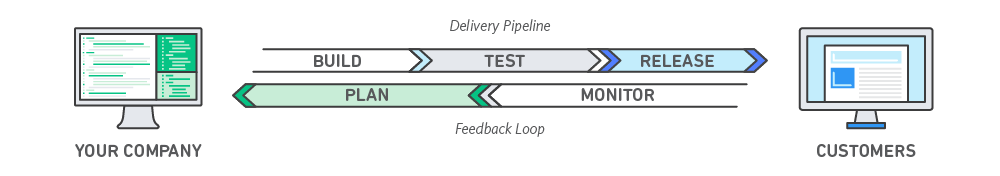
\includegraphics[width=1\linewidth]{figura1}
	\caption{Ciclo DevOps}
	Fonte: AWS
	\label{fig:figura1}
\end{figure}

As implementações nesse tipo de ambiente fazem uso de ferramentas de automação com o intuito de dinamizar cada vez mais a infraestrutura e torná-la mais programável, de forma que reflita na melhoria contínua da comunicação e integração entre desenvolvedores e administradores de infra, transformando o cenário tradicional de isolamento entre essas duas equipes em um ambiente participativo e colaborativo.

			\begin{flushright}
				\begin{minipage}{0.75\textwidth}
					\normalsize "Seu objetivo é criar uma cultura de colaboração entre as equipes de desenvolvimento e de operações que permite aumentar o fluxo de trabalho completado $($maior frequência de deploys$)$ ao mesmo tempo aumentando a estabilidade e robustez do ambiente de produção." (SATO, 2016).
				\end{minipage}
			\end{flushright}


O DevOps representa muito mais do que simplesmente o uso de ferramentas de automação, é importante observarmos que trata-se de uma quebra de paradigmas e uma mudança na cultura no negócio, uma nova forma de entrega e produção.

			\begin{flushright}
				\begin{minipage}{0.75\textwidth}
					\normalsize "Mais do que uma modernização tecnológica, por meio das mais diversas áreas de inovação, é uma oportunidade de evoluir a cultura e os processos da organização." (COSTA, 2017).
				\end{minipage}
			\end{flushright}

A agilidade no processo de deploys citado anteriormente aluz à uma necessidade de amparo para que essa entrega rápida de fato aconteça, e mais do que isso, a demanda por parte dos clientes ou usuários de determinada aplicação, requer cada vez mais velocidade no uso de determinada funcionalidade. Analogamente à revolução industrial do século XX, a mudança na forma de produção de produtos naturalmente está sendo absorvida pela tecnologia, assim, a concepção desse produto deve acompanhar a demanda externa. Nesse sentido, a adaptabilidade e mudança da arquitetura funcional no desenvolvimento de serviços tecnológicos são necessidades relevantes, a cultura DevOps é uma mudança importante nesse ponto.

Segundo uma pesquisa realizada pelo Gartner Group sobre DevOps, em 2015, somente 29\% das organizações pesquisadas tem o modelo atuante em produção. É evidenciado ainda que apenas 42\% desses, tem a atuação do DevOps em aplicações móveis.
%Fonte: https://www.itforum365.com.br/tecnologia/como-devops-pode-ser-usado-para-desenvolvimento-de-aplicacoes-moveis/

De acordo com o mesmo grupo o DevOps evoluiria de uma estratégia de nicho para uma estratégia comum sendo empregada por 25\% das organizações do Global 2000\footnote{Forbes Global 2000 é uma classificação anual das 2.000 empresas públicas do mundo pela revista Forbes. O ranking é baseado em quatro critérios: vendas, lucro, ativos e valor de mercado. A lista é publicada desde 2003. Fonte: Wikipédia}.

O uso da cultura DevOps deve ser absorvida na necessidade de versionamento contínuo de determinada aplicação, ou seja, a frequente execução de deploys. Nisso, é importante observarmos que a rápida proliferação de software requer atualizações operando na mesma medida ágil e demanda pela competitividade de mercado, visto que a velocidade no atendimento da expectativa dos clientes diferencia a empresa em relação às demais atuantes no mercado.


% ############# PESQUISAR E ACRESCENTAR (Ver com o professor)  #######################
%- Levantamento de tarefas com fim na automatização;
%- Definir ferramentas adotadas;
%- Pesquisar sobre práticas ágeis que facilitem o gerenciamento.
% ####################################################################################

A principal vantagem no uso de DevOps é a melhora evidente nos processos e automatização das tarefas, otimizando o tempo e reduzindo os ciclos de desenvolvimento. Por se tratar de uma interação entre as equipes de desenvolvedores e operacionais, dizemos que é um sistema bimodal de trabalho.

O monitoramento de métricas e registro de logs é um aspecto relevante. Leva-se em conta que os serviços devem estar disponíveis 24 horas por dias e durante os 7 dias da semana, acarretando em uma massiva análise de dados e logs gerados pelo sistema, portanto, a rotina na observância desses elementos deve ser constante. É possível, inclusive, a criação de alertas que apontem situações e permitam a gerência proativa dos serviços.

Outro benefício fundamental do DevOps é o aumento na comunicação e colaboração que envolve todos os personagens da empresa. É importantíssimo a definição de normas que permitam um maior compartilhamento de informações, ou que permitam a proliferação da comunicação sejam por meio de qualquer que for o método ou tecnologia, desde que agregue valor. Além disso, a diminuição de ruídos na comunicação e conflitos entre as equipes melhora o ambiente e tende a produzir efeitos positivos ao fim do processo.

Podemos ainda elencar ganhos em maior estabilidade e melhor desempenho, e tão importante quanto, a redução considerável de custos de trabalho, visto que a diminuição de tempo de produção e menor esforço afeta diretamente o custo estimado em um projeto.


\section{Infraestrutura como Código}
Falar em infraestrutura com código é exatamente absorver o entendimento do tratar a estrutura de TI como um software, programável. Como isso é possível o uso de práticas que envolvam o controle por versionamento, testes automatizados, entrega contínua, entre diversos outros recursos.

O uso de práticas anteriores com métodos de gerenciamento de infraestutura forma válidos e deram uma base poderosa para a concepção de novas tecnologias. Atualmente, a constante demanda de software cada vez mais dinâmicos e alto índice de deploys, inclusive simultâneos, levam à necessidade de concepção de uma infraestrutura que acompanhe o ritmo de complexidade dos sistemas de aplicação.



\section{Principais Ferramentas e Recursos Tecnológicos Disponíveis}
Apesar do conceito DevOps ser recente, a gama de ferramentas que contribuem para implantação dessa cultura já se mostram bastante diversificadas. Dentre as mais comuns podemos apresentar:

\subsection{Atlas}
É uma ferramenta disponibilizada pela Hashicorp, que tem a função de unificar projetos open source para o manejo de aplicações finalizadas no desenvolvimento para a produção em qualquer que seja a infraestrutura.
As etapas do Atlas seguem cinco passos (Figura 2), isso independe da tecnologia utilizada, sejam máquinas virtuais ou contêineres, as etapas se mantêm as mesmas.

\begin{figure}[htb]
	\centering
	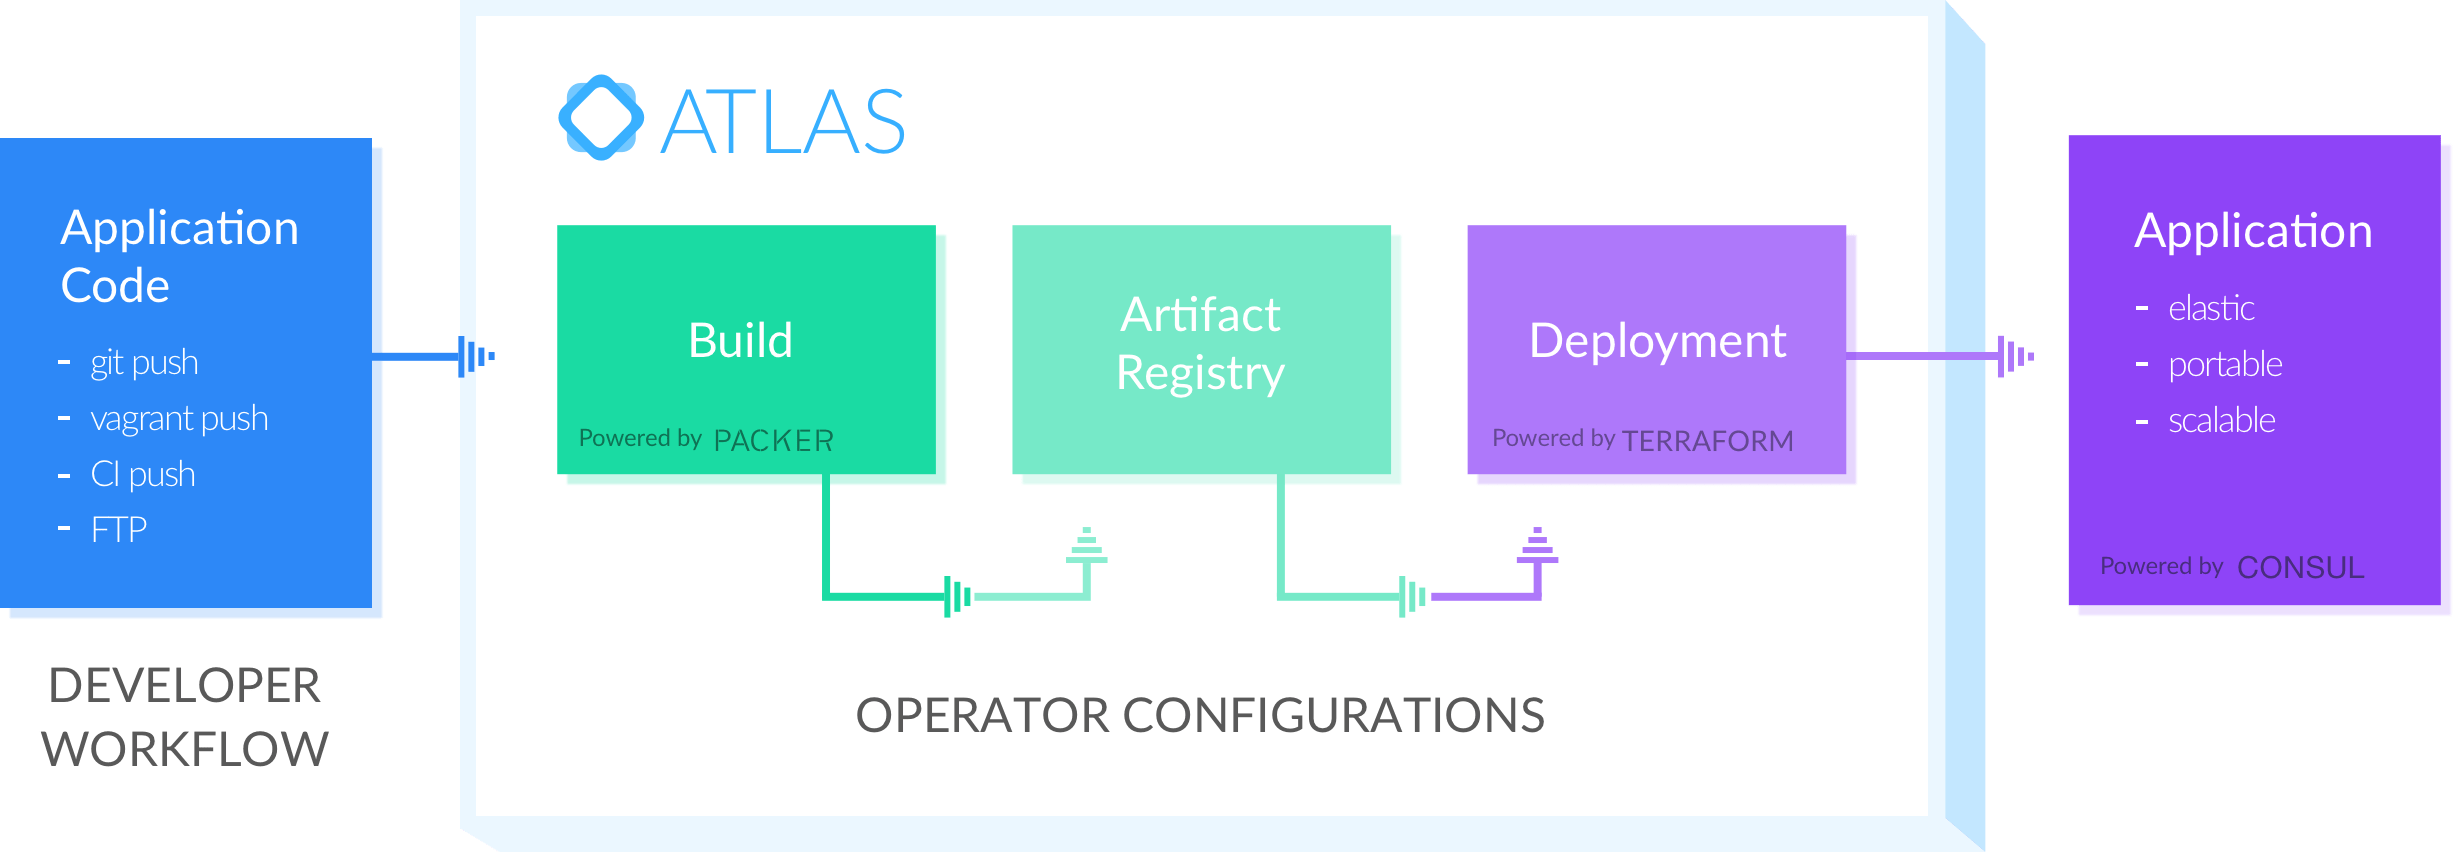
\includegraphics[width=0.8\linewidth]{etatasAtlas}
	\caption{Etapas do Atlas}
	Fonte: Hashicorp
	\label{fig:etatasAtlas}
\end{figure}

O Atlas não é um software de caixa preta, ou seja, é possível acesso a serviços que contribuem para tanto, como Vagrant (gerencia ambientes de desenvolvimento), Packer (construção de artefatos), Terraform (implantação de Infraestrutura) e Consul (monitora os serviços em tempo real).

\subsection{Chef}
É um framework destinado à automatização para sistemas e infraestrutura em nuvem. O Chef\footnote{Disponível em https://www.chef.io} constrói, entrega e administra fazendo uso de scripts replicáveis.

O Chef tira a carga dos administradores de sistemas que focam no gerenciamento projetado para servidores autônomos, ele permite executar cetenas de instâncias de servidor em um tempo imensamente maior se comparado ao uso comum em deploys.

Para gerenciar esse tipo de configuração, o Chef, transforma a infraestrutura em código, deixando o processo mais flexível, legível pelos analistas e testável, possibilitando assim a gerência de recursos tanto localmente quanto na nuvem

Em sua topologia o Chef tem três principais componentes: o Servidor Chef, as Estações e o Nós.

O maior atrativo dessa ferramenta é o uso de "cookbooks" ou receitas, são ditas configurações plugáveis, que envolvem todas as instalações e parâmetros necessários para atender determinada aplicação no servidor ou máquina. Assim como as receitas convencionais definem uma estrutura sequencial que deve ser seguida a fim de tornar o produto final reflexo de uma ideia original, o Chef mantém um conceito semelhante a isso, onde define-se um estado desejado do sistema, desenvolvendo um código de configuração, então o ele processa esse código, une ao processo os dados do nó em questão e garante que o estado concebido seja correspondente ao estado do sistema. 

O Chef pode ser executado em várias plataformas, como Windows, distribuições Linux, FreeBSD, Solaris, AIX, Cisco IO e Nexus. E ainda suporta plataformas em nuvem,como Amazon Web Services $($AWS$)$, Google Cloud Platform, OpenStack, IBM Bluemix, HPE Cloud, Microsoft Azure e VMware vRealize.

\subsection{Docker}

O Docker\footnote{Disponível em https://www.docker.com/}. é uma plataforma de automação que implanta as aplicações em espaços isolados chamados de \textit{containers}, possibilitando as executarem as aplicações de forma mais ágil. O objetvo é criar múltiplos ambientes dentro de um mesmo servidor, acessíveis externamente.

Segundo Matthias e Kane, no livro Primeiros Passos com Docker: 
%Colocar o parágrafo abaixo como citação

			\begin{flushright}
				\begin{minipage}{0.75\textwidth}
					\normalsize "... o Docker influencia a arquitetura do software no sentido de encorajar aplicações trabalhadas de modo mais robusto. Sua filosofia de arquitetura gira em torno de contêineres atômicos ou descartáveis. Durante a implantação, todo ambiente sobre o qual a aplicação antiga roda é jogado fora com ela. Nada no ambiente da aplicação viverá mais do que a aplicação em si; essa é uma pequena ideia com grandes repercussões." (MATTHIAS e KANE, 2015)
				\end{minipage}
			\end{flushright}

O Docker é uma plataforma Open Source, que não pode ser confundido com um ambiente tradicional de virtualização. No Docker fazemos uso de recurso isolados que utilizam bibliotecas do kernel em comum, isso porque é presente nessa ferramenta o Linux Containers (LXC).

Com ele é possível empacotar a aplicação ou um ambiente em um contêiner e movê-lo para qualquer outro host que possua o Docker instalado, tornando assim uma ferramenta portável. A grande vantagem disso é que não há necessidade de reconfigurar todo o ambiente novamente, visto que todo ele é movido, reduzindo acentuadamente o tempo de deploy de uma infraestrutura.

Essa plataforma não pode ser confundida com um ambiente virtualizado, visto que em cenários que utilizam máquinas virtuais há a presença de uma camada intermediária de sistema operacional entre o host e as aplicações, no Docker essa é desnecessária pois ele não utiliza kernel, tornando independente quanto a nível de disco, memória e processamento.

A infraestrutura no Docker também é replicável, é possível criar imagens predefinidas e disponibilizá-las em ambientes de desenvolvimento, teste, homologação e produção para aplicações.


\subsubsection{Vantagens:}
Podemos elencar alguns ganhos consideráveis na utilização do Docker:
\begin{itemize}
\item Empacotamento de software otimizando o uso das habilidades dos desenvolvedores;
\item Empacotamento de aplicação de software com todos os arquivos e dependências necessárias para determinada aplicação.
\item Utilização de artefatos empacotados que possibilitem a passagem pelo teste e produção sem necessidade de recompilação.
\item Uso de softwares sem onerar recursos demasiados, visto que o contêiner é apenas um processo que se comunica diretamente com kernel do Linux.
\end{itemize}

\begin{figure} [htb]
	\centering
	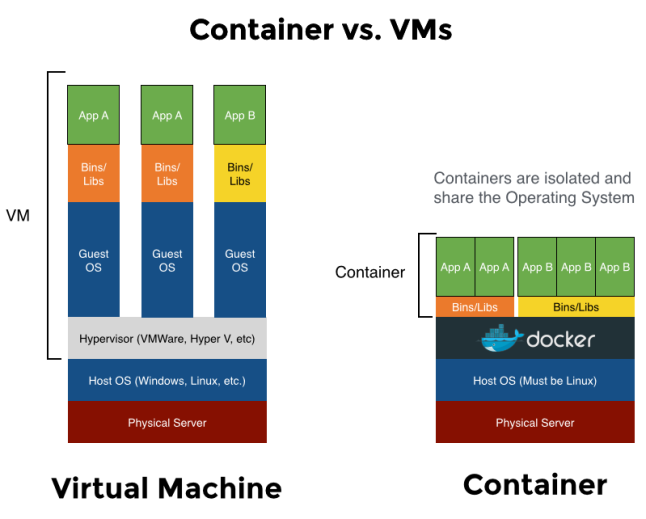
\includegraphics[width=0.55\linewidth]{imagens/dockerXvm}
	\caption{Comparativo Docker x Máquinas Virtuais}
	\label{fig:dockerXvm}
\end{figure}

\subsection{Puppet}
É uma ferramenta de código livre para gestão de configurações. A ideia central do Puppet\footnote{Disponível em https://www.puppet.com/} é a administração de diversas máquinas físicas ou virtuais, onde a configuração é centralizada em um único nó e então distribuídas por diversos nós na rede, assim, gerenciando configurações, automatizando instalação de pacotes e facilitando o estabelecimento de normas e auditoria.

A ferramenta está disponível em duas versões: Puppet Enterprise $($com suporte pago$)$, e a Open Source Puppet $($código aberto$)$. É uma ferramenta bem utilizada pela comunidade e por isso existem muitos módulos desenvolvidos, empresas como McAfee e Nasa fazem uso dela.

O Puppet utiliza SSH para a conexão aos hosts, esse é um ponto positivo se olharmos pela ótica que em alguns cenários não é possível a instalação de agentes ou em situações onde o agente consome uma fatia considerável de memória e cpu.



\begin{figure} [htb]
	\centering
	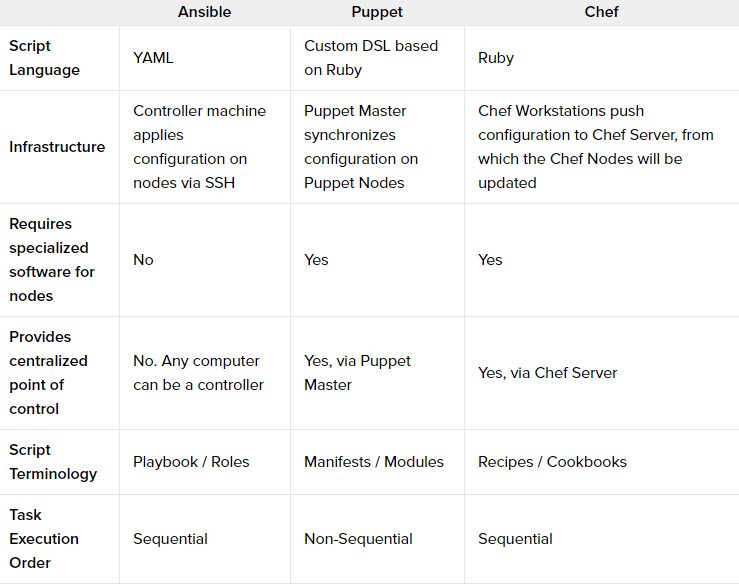
\includegraphics[width=0.7\linewidth]{puppet}
	\caption{Comparativo entre Ferramentas de Gerenciamento de Configurações}
	Fonte: Digital Ocean
	\label{fig:puppet}
\end{figure}


\subsection{Ansible}

O Ansible\footnote{Disponível em https://www.ansible.com} foi criado em 2012, por Michael DeHann, basicamente essa ferramenta gerencia configurações e orquestra tarefas. 

Nesse sentido ele implementa módulos para nós sobre SSH. Os módulos são distribuídos nos nós temporariamente que realizam a comunicação com a máquina de controle (assim com em ferramentas concorrentes) por meio de um protocolo JSON.
O diferencial do Ansible em relação as demais ferramentas que se propõe ao mesmo objetivo, é que ele atua com uma arquitetura cliente-servidor, sem agente,  isso que dizer que os nós não são necessários para a instalação dos daemons para comunicação com a máquina controle. Isso resulta em diminuição de carga na rede. 

			\begin{flushright}
				\begin{minipage}{0.75\textwidth}
					\normalsize "Os principais objetivos do Ansible são a simplicidade e facilidade de uso. Ele também tem um forte foco na segurança e confiabilidade, com um mínimo de peças móveis, o uso do OpenSSH para o transporte (com um modo acelerado e modos alternativos) é uma linguagem projetada em torno auditabilidade por seres humanos, mesmo para aqueles que não são familiarizados com o programa." (ANSIBLE, Inc. 2016). 
				\end{minipage}
			\end{flushright}

O Ansible oferece duas versões, o Ansible Core, que é a versão gratuita e de código aberto, e o Ansible Tower, versão comercial.

Nessa ferramenta ainda encontramos o uso de um arquivo de inventário, denominado "hosts", que definem quais nós serão gerenciados, que é simplesmente um arquivo de texto que lista os nós individualmente ou agrupados ou até um arquivo executável que constrói um inventário de hosts.

Na forma tradicional de trabalho o Ansible faz o upload do código que deve ser executado nas estações clientes, é então executado, retorna o resultado da execução e após isso é removido dos clientes.

Quando usamos a ótica DevOps esse tipo de fluxo é modificado, fazendo uso do protocolo NETCONF $($RFC 6241$)$, onde é possivel o envio de comandos aos componentes e receber o retorno da aplicação.

\subsubsection{Componentes:}
O Ansible é estruturado pela composição dos seguintes elementos:

\begin{itemize}
	\item Playbooks\footnote{Disponível em https://docs.ansible.com/ansible/playbooks.html}: arquivos de configuração, implementação e linguagem de orquestração do Ansible.
	\item Agentless\footnote{Disponível em https://dbruno.ansible.com/ansible/}: É descartado o uso de agente nos servidores a serem monitorados. Isso deve-se à utilização de OpenSSH para definir o estado atual do ambiente, adaptando-se se acaso estiver em desconformidade com a configuração no playbook.
	\item Módulos\footnote{Disponível em https://docs.ansible.com/ansible/modules.html}: São as tarefas executadas de fato. Os módulos são ditos como "plugins de tarefas" e por isso são eles que realizam as atividades pertinentes.
	\item Inventário\footnote{Disponível em https://dbruno.ansible.com/ansible/}: Armazena e controla informações sobre os grupos de hosts.
\end{itemize}

\subsubsection{Vantagens:}
Podemos apontar alguns ganhos consideráveis na utilização do Ansible:
\begin{itemize}
	\item Não há a necessidade na instalação de agentes nos servidores a serem gerenciados;
	\item Gerencia paralela e simultaneamente de forma orquestrada; 
	\item Simples configuração e bem estruturado;
	\item Desenvolvimento em diversas linguagens.
\end{itemize}

\subsection{GITHUB}
É um dos serviços web mais difundidos. Com essa ferramenta é possível hospedar projetos e aplicações, trabalhando com controle de versionamento.

O Github\footnote{Disponível em https://www.github.com} funciona por meio de repositórios, que funcionam como pastas e dentro destas outras pastas que comportam os arquivos de diversas extensões e linguagens. Ainda oferece a possibilidade de contribuir com um determinado para o desenvolvimento de determinado projeto. Além, e permitir o acesso múltiplo por diversos desenvolvedores de um mesma empresa, permitindo que vários programadores trabalhem simultaneamente em uma mesma aplicação ou arquivo.

\begin{figure} [htb]
	\centering
	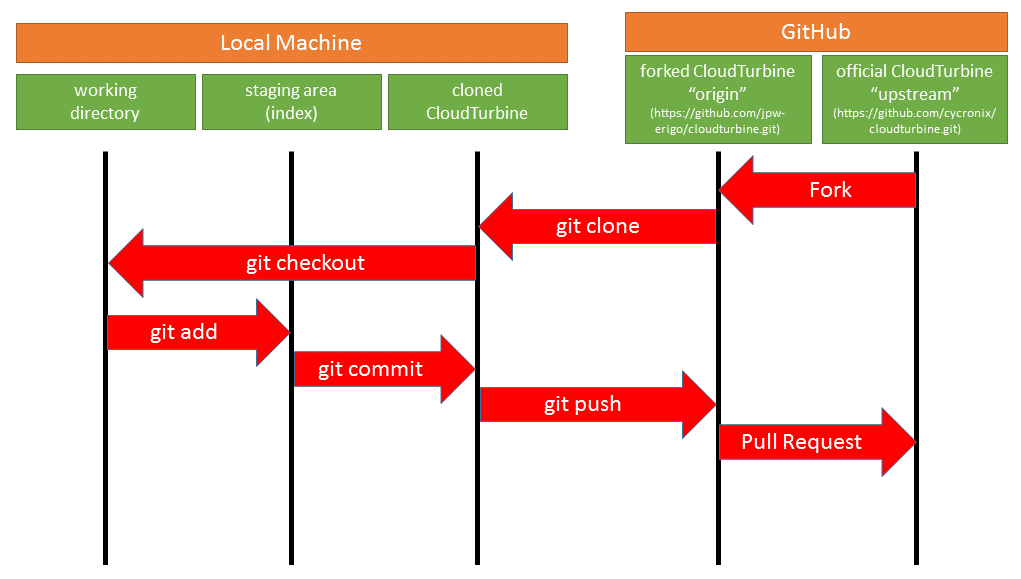
\includegraphics[width=0.7\linewidth]{git}
	\caption{Fluxo commit e request}
	Fonte: Cloud Turbine
	\label{fig:git}
\end{figure}

\subsection{Jenkins}
Essa ferramenta multiplataforma e funciona como um servidor destinado a integração contínua que automatiza a execução de tarefas, possui código aberto e permite ao usuário total liberdade em sua operação.

O Jenkins\footnote{Disponível em https://www.jenkins.io} pode ser integrado ao Git, SVN, CVS, Maven, entre outros. É importante ressaltar que um ponto forte do Jenkins é a difusão entre a comunidade.

Um recurso interessante é o uso de Forks $($recurso do GitHub$)$, que permitem a criação de cópias de um determinado projeto e trabalha nesse sem a preocupação de afetar em algum ponto a aplicação original.

É possivel ainda, adicionar testes de desempenho e balanceamento na integração contínua, permitindo a análise de risco e a reduzir eventuais quedas de performance no momento em que um novo recurso é adicionado ou a correção de um erro presente.

% ############ ADICIONAR DIAGRAMA (VER COM O PROFESSOR)





% ---
% Capitulo de METODOLOGIA
% ---




\chapter{Metodologia}\label{cap:metodologia}
Para o desenvolvimento deste trabalho, com foco em atendimento aos seus objetivos, far-se-á uso de softwares open source  $($código livre$)$, que possibilitam a utilização gratuita dos mesmos, tendo suporte contínuo da comunidade, além de permitir alterações em sua estrutura, acaso sejam necessárias e relevantes.




\subsection{Ferramentas Utilizadas}
Para concepção desse trabalho serão adotadas as seguintes ferramentas:

\begin{itemize}

\item Github: Versionamento e repositório;

\item Ansible: Gerenciador de configuração;

\item Jenkins: Automatização de execução de tarefas.
\end{itemize}


\section{Materiais}






\section{Implementação dos métodos}




\chapter{Resultados}\label{cap:resultados}
\section{Introdução}





\chapter{Conclusão}\label{cap:conclusao}


% ----------------------------------------------------------
% ELEMENTOS PÓS-TEXTUAIS
% ----------------------------------------------------------
\postextual
% ----------------------------------------------------------

% ----------------------------------------------------------
% Referências bibliográficas
% ----------------------------------------------------------
\bibliography{bibliografia}

% ----------------------------------------------------------
% Glossário
% ----------------------------------------------------------
%
% Consulte o manual da classe abntex2 para orientações sobre o glossário.
%
%\glossary

%---------------------------------------------------------------------
% INDICE REMISSIVO
%---------------------------------------------------------------------
\phantompart
\printindex
%---------------------------------------------------------------------

\end{document}
\grid
